%%%%%%%%%%%%%%%%%%%%%%%%%%%%%%%%%%%%%%%%%%%%%%%%%%%%%%%%%%%%%%%
%
% Welcome to Overleaf --- just edit your article on the left,
% and we'll compile it for you on the right. If you give
% someone the link to this page, they can edit at the same
% time. See the help menu above for more info. Enjoy!
%
%%%%%%%%%%%%%%%%%%%%%%%%%%%%%%%%%%%%%%%%%%%%%%%%%%%%%%%%%%%%%%%
%
% For more detailed article preparation guidelines, please see:
% http://f1000research.com/author-guidelines

\documentclass[10pt,a4paper,twocolumn]{article}
\usepackage{f1000_styles}
\usepackage{url}

%% Default: numerical citations
% \usepackage[numbers]{natbib}

%% Uncomment this lines for superscript citations instead
% \usepackage[super]{natbib}

%% Uncomment these lines for author-year citations instead
\usepackage[round]{natbib}
\let\cite\citep

\begin{document}

\title{iSEE: Interactive SummarizedExperiment Explorer}
\titlenote{The title should be detailed enough for someone to know whether the article would be of interest to them, but also concise. Please ensure the broadness and claims within the title are appropriate to the content of the article itself.}
\author[1,$\dagger$]{Kevin Rue-Albrecht}
\author[2,3,$\dagger$]{Federico Marini}
\author[4,$\dagger$]{Charlotte Soneson}
\author[5,$\dagger$,$\ast$]{Aaron T. L. Lun}

\affil[1]{Kennedy Institute of Rheumatology, University of Oxford, Oxford OX3 7FY, United Kingdom}
\affil[2]{Center for Thrombosis and Hemostasis (CTH), University Medical Center of the Johannes Gutenberg University Mainz, Mainz}
\affil[3]{Institute for Medical Biostatistics, Epidemiology and Informatics (IMBEI), University Medical Center of the Johannes Gutenberg University Mainz, Mainz}
\affil[4]{University of Zurich and SIB Swiss Institute of Bioinformatics, Zurich, Switzerland}
\affil[5]{Cancer Research UK Cambridge Institute, University of Cambridge, Cambridge CB2 0RE, United Kingdom}
\affil[$\dagger$]{These authors contributed equally.}
\affil[$\ast$]{To whom correspondence should be addressed.}


\maketitle
\thispagestyle{fancy}

% Please list all authors that played a significant role in the research involved in the article. Please provide full affiliation information (including full institutional address, ZIP code and e-mail address) for all authors, and identify who is/are the corresponding author(s).
% TODO: full address and emails too? if so, in which format do we provide them?

\begin{abstract}

\textbf{Summary:} Data exploration is critical to the comprehension of large biological datasets generated by high-throughput assays such as sequencing.
However, most existing tools for interactive visualization are limited to specific assays or analyses.
Here, we present the iSEE (Interactive SummarizedExperiment Explorer) software package, which provides a general visual interface for exploring data in a SummarizedExperiment object.
iSEE is directly compatible with many existing R/Bioconductor packages for analyzing high-throughput biological data,
and provides useful features such as simultaneous examination of multiple data aspects, dynamic linking between plots and code tracking for reproducibility.
We demonstrate the utility and flexibility of iSEE by applying it to explore a range of real transcriptomics and proteomics datasets.\\
\textbf{Availability:} iSEE is publicly available as an R package from the open-source Bioconductor project (\url{https://bioconductor.org/packages/iSEE}).\\
\textbf{Contact:} aaron.lun@cruk.cam.ac.uk\\
\textbf{Supplementary information:} Supplementary data are available online.

% Abstracts should be up to 300 words and provide a succinct summary of the article. Although the abstract should explain why the article might be interesting, care should be taken not to inappropriately over-emphasize the importance of the work described in the article. Citations should not be used in the abstract, and the use of abbreviations should be minimized. If you are writing a Research or Systematic Review article, please structure your abstract into Background, Methods, Results, and Conclusions.


\end{abstract}

\section*{Keywords}

% Please list up to eight keywords to help readers interested in your article find it more easily.

Single-cell, gene expression, transcriptomics, proteomics, visualization, interactive, shiny, Bioconductor

% TODO: refine keywords

\clearpage

\section*{Introduction}
Interactive data exploration is critical to the analysis and comprehension of the data generated by high-throughput biological assays such as transcriptomics.
Exploration drives the formation of novel data-driven hypotheses prior to a more rigorous statistical analysis, and enables diagnosis of potential problems such as batch effects and low-quality samples.
To this end, visualization of the data in an intuitive and interactive interface is crucial, allowing researchers to examine the data from different perspectives across samples (e.g., experimental replicates, patients, single cells) and features (e.g., genes, transcripts, proteins, genomic regions, microarray probe sets).

Most existing tools for interactive visualization of biological data are designed for specific assays and analyses, e.g., pRoloc for proteomics \citep{gatto2014mass}, shinyMethyl for methylation \citep{fortin2014shinymethyl}, HTSvis for high-throughput screens \citep{scheeder2017htsvis}.
Opportunities for customization are generally limited, making it difficult to re-use the same visualization software for new technologies or experimental designs where different aspects of the data are of interest.
Moreover, standalone tools such as the Loupe Cell Browser from 10X Genomics \citep{zheng2017massively} do not easily integrate into established analysis pipelines such as those based on the R statistical programming language \citep{rcore2008R}.
This complicates any coordinated use of these tools with a reproducible, transparent, and statistically rigorous analysis.

\begin{figure*}[t]
\includegraphics[width=\textwidth]{pics/Fig1.pdf}
\caption{iSEE uses a customisable multi-panel layout (A) that simultaneously displays one or more panels of various types, where each panel type visualizes a different aspect of the data.
New panels of any type can be added (i), and all panels can be removed, reordered or resized (ii).
Panel types are available to visualize sample-based reduced dimensionality embeddings (iii), sample-level metadata (iv), and experimental observations across samples for each feature (v).
For these panel types, each sample is represented as a point, which can be coloured according to sample-level metadata or feature-level observations.
Depending on whether the variables of interest are categorical or numeric, panels will automatically switch between scatter plots, violin plots or ``rectangle plots'' (where each combination of categorical levels is represented by a rectangle with area proportional to the frequency of combination).
Other panel types include row statistics tables (vi), to facilitate searching across features and their metadata; heatmaps (vii), to visualize experimental observations for multiple features; and feature-level metadata plots.
(B) Information can be transmitted between panels according to a user-specified scheme.
Here, the selection of feature $X$ in the row statistics table determines the y-axis of the feature expression plot, and colours the samples in the reduced dimension plot by the expression of $X$.
Selection of points in the reduced dimension plot (dotted blue line) also determines the samples that are shown in the column data (i.e., sample metadata) plot;
further selection of points in the column data plot determines the samples that are shown in the heatmap.
}
\label{fig:iSEE}
\end{figure*}

\section*{Implementation}
Here, we present the iSEE software package for interactive data exploration.
iSEE is implemented in R using the Shiny framework \citep{chang2017shiny} and exploits data architectures from the open-source Bioconductor project \citep{gentleman2004bioconductor}.
The iSEE interface is initialized with a single function call accepting a SummarizedExperiment object as input \citep{huber2015orchestrating}.
The SummarizedExperiment class stores one or more matrices of experimental observations as ``assays'', where rows and columns represent genomic features and biological samples, respectively.
For instance, individual assays may represent gene expression matrices of raw counts along with different normalization strategies.
In addition, per-feature or per-sample variables are stored in the ``rowData'' and ``colData'', respectively; those may include experimental metadata as well as any analysis results.
All of these data aspects can be readily examined alongside one another in the multi-panel layout of the iSEE interface (Fig.~\ref{fig:iSEE}A).

Notably, the flexibility of the SummarizedExperiment class is the driving factor behind its broad deployment throughout the Bioconductor ecosystem, with uses in RNA sequencing \citep{love2014moderated}, methylation \citep{aryee2014minfi} and Hi-C analysis pipelines \citep{lun2016infrastructure}, amongst others.
As a consequence, the widespread adoption of the SummarizedExperiment class and its specialized extensions such as the SingleCellExperiment class enables iSEE to offer immediate interactive visualization for a variety of data modalities, complementing the state-of-the-art analysis workflows and methodologies already available in R/Bioconductor packages.
%In particular, we leverage off the state-of-the-art allowing us to avoid re-implementing them in iSEE (as is commonly done in other standalone visualization tools).
% KRA: any other child class like SingleCellExperiment worth mentioning? e.g. the BSseq class

% \section*{Description of the iSEE interface} % FM: if required, "turn on the section"?
The layout of the iSEE user interface is built using the shinydashboard package \citep{chang2018shinydashboard}.
The header contains three dropdown menus that provide constant access to diagnostics of the current application state, documentation, and additional information, respectively. % TODO, FM: maybe we can/should cross-reference to the upcoming sections?
The sidebar of iSEE contains a menu enabling the creation of new plots and tables (referred to as ``panels'') in the interface.
Individual color-coded tabs allow the corresponding panel to be re-ordered, adjusted in width and height, or removed from the user interface.
The main component of the iSEE interface displays a combination of active panels controlled by the user's actions in the current session.
Notably, individual panels can optionally be linked to one another, allowing information to be dynamically transmitted between the panels.
In addition to the package documentation and vignette, users can familiarize themselves with the main elements of the user interface by taking an interactive tour (based on the rintrojs package []ganz[]), allowing them to learn the basic usage mechanisms by doing.


\section*{Functionalities}
Currently, six different types of panels can be generated with iSEE. For each panel, three different set of parameters are available in collapsible boxes: namely, Data parameters control the sources of information specific to each type of plot; Visual parameters direct the appearance of the data points (e.g. color, opacity, size); and Selection parameters adjust the behaviour of point selections transmitted between linked panels.

Individual panel types include:

\begin{itemize}
\item Reduced dimension plots -  Display any two dimensions from precomputed reduced dimension matrices (e.g., PCA, t-SNE) available in the reducedDim slot of a SingleCellExperiment object supplied to iSEE. Notably, the capacity of SingleCellExperiment objects to store any number of reduced dimension matrices enables efficient exploration of high-dimensional datasets.
\item Column data plots - Visualize sample metadata stored in the colData slot of SummarizedExperiment object. Conveniently, both categorical and continuous covariates are seamlessly supported, with the geometry of the plot layers automatically switching between scatter plots, violin plots, or bi-categorical grid plots, according to the nature of the data on both axes.
\item Feature expression plots - Visualize expression values from any assay stored in the SummarizedExperiment object for a particular feature (e.g., gene, protein) within individual samples.
This type of plot often adopts a violin or scatter plot geometry, according to the nature of the second covariate.
\item Row statistics tables - Present the contents of the rowData slot for the SummarizedExperiment object.
These tables are particularly helpful when dynamically linked with other panels, both as summary tables of selected genes and sources of selections to visualise or color in target plots.
\item Row data plots - Visualize the information stored in the rowData slot of a SummarizedExperiment object, following an implementation similar to column data plots.
\item Heat maps - Simultaneously visualize assay data and sample metadata, in the form of color-coded expression matrix where rows represent features and columns represent samples.
As such, heat maps may receive both row and column data inputs from appropriately linked panels, to control the subsetting and highlighting of individual features and samples selected in the respective source panels.
\end{itemize}

The color of individual data points (i.e., samples) can be controlled in different ways in each plot. The default is no color scheme, with the same color (default, black) being applied uniformly to all data points.
However, any column from the metadata available in the SummarizedExperiment may be used, as well as any any assay data. The plotting routines automatically adjust the scale to use, based on the chosen variable.

\subsection*{Dynamic linking between panels}
A key feature of iSEE is the ability to dynamically transmit information between panels (Fig.~\ref{fig:iSEE}B).
Users can define arbitrary links between ``transmitting'' and ``receiving'' panels, whereby selections in transmitting tables and plots highlight the corresponding data points in receiving panels.
This feature facilitates exploration of the relationships between different aspects of the data -- for example, users can easily determine co-expression patterns of genes in a particular region of a reduced dimensionality embedding, by transmitting information from the reduced dimension plot to one or more feature expression plots.
The linking paradigm extends to multiple plots whereby a plot can transmit to multiple receivers, or a receiving plot can itself transmit its own selection to another plot.
This allows users to mimic the arbitrarily complex gating strategies often found in analyses of flow cytometry data \citep{finak2014opencyto}, with the advantage of being extensible to any (meta)data present in a SummarizedExperiment object.
Information can similarly be transferred between tables and plots, e.g., selecting a row determines how points are coloured in receiving plots.

\subsection*{Advanced features and customization}

Additional parameters, provided when launching the iSEE application, can customize the startup state of the application
The number and identity of the panels, as well as their inter-relationships can also be specified at initialization, thus avoiding the need to click through the choices to obtain the desired panel setup.
An example of such customization is provided in %% TODO %%
Users can refer to the documentation of ?defaults for the full list of values that can be specified in iSEE.


\subsection*{ExperimentColorMap: custom color maps}

iSEE also offers a host of other customizable features to improve data exploration.
Users can supply their own colour mappings to iSEE, to control how colour scales are chosen for each metadata variable and assay type across all panels in the application.
% TODO: KRA develop here

\subsection*{Linked feature annotations}

Row statistics tables can be augmented with dynamic annotation based on the selected row, linking to online resources such as Ensembl or Entrez. % do we need to cite them? at least ENSEMBL has updated citable papers

\subsection*{Density-dependent downsampling for speed}

For large datasets, points can be downsampled in a density-dependent manner to accelerate rendering of the plots, improving the responsiveness of the interface without compromising the fidelity of the visualization.

\subsection*{Code tracking and reproducibility}

iSEE also automatically memorizes the exact R code that was used to generate every plot and the existing links, extending previous work by \cite{marini2016interrepro}. A modal popup window, with a shinyAce-based text editor, where the code is formatted and displayed with syntax highlighting, is opened when clicking on the `Extract the R code'' button from the diagnostics dropdown menu in the header.
This allows users to easily reproduce the results of any exploratory analysis, simply by copying the code reported by iSEE into their own analysis scripts.
Additionally, the ``Examine panel chart'' functionality, in the iSEE diagnostics dropdown menu, returns a graph representation of the existing links and point selection among the open panels. This can be very useful in sessions that include a large number of panels.
Clicking on the ``Display panel settings'' button from the same dropdown menu returns the required lines of code that underlie the current setup of currently open panels.

\subsection*{App tours and deployment}
After analyses are completed, users can deploy iSEE on a server with a bespoke step-by-step ``tour'' of their dataset, guiding the audience through an examination of the salient features in the data.
This normally requires the setup of a Shiny Server, % TODO: FM, do we want to provide some basic instructions on how to do it?,
as well as the preparation of the dataset at hand in form of a SummarizedExperiment - which many workflows available in Bioconductor adopt as main representation.
Tours can be provided to the iSEE function in the form of simple data frames, containing the list of DOM elements in the Shiny app to anchor the corresponding descriptions.
Examples of such tours can be found in the inst/extdata folder of the iSEE package, as well as in the GitHub repository of this manuscript, \url{https://github.com/LTLA/iSEE2018/tree/master/tours}.


%\section*{Demonstration data sets and tours}
\section*{Use cases} % FM: used often in other software articles in F1000res
To demonstrate the functionality and flexibility of the iSEE package, we applied our method to a number of publicly available datasets.
Details are provided in the tour subfolder of the GitHub repository for this manuscript (\url{https://github.com/LTLA/iSEE2018}), and for each dataset a combination of \_app.R and \_tour.txt is provided.
An instance of iSEE running on the respective datasets is provided as a stand-alone webpages, for demonstration purposes without the need of software installation.

\subsection*{Single-cell plate-based RNA-seq}
% TODO: better title, or do we drop this allen section altogether?
We demonstrate the application of iSEE to examine a subset of 379 cells from of mouse visual cortex \citep{tasic2016allen}.
This example can be reproduced also by calling

library(iSEE)
example(iSEE, ask = F)

% TODO: embed the allen demo data set
\url{http://shiny.imbei.uni-mainz.de:3838/iSEE/}

\subsection*{Single-cell droplet-based RNA-seq}
% TODO: better title, or do we drop the allen section altogether (above)?
We also demonstrate the use of iSEE to explore a larger data set of 4,000 PBMC single-cell RNA sequencing dataset from 10X Genomics \citep{zheng2017massively}.
% TODO: take out the juice from what the tour does, and maybe one figure/screenshot in each case?
% embed the allen demo data set
\url{http://shiny.imbei.uni-mainz.de:3838/iSEE_PBMC4k/}

\subsection*{Bulk RNA-seq from TCGA}
We also demonstrate how iSEE seamlessly scales up with larger data sets as the TCGA RNA-seq collection of measurements for 23,368 genes across 7,706 tumor samples \citep{piccolo2015TCGA}.
% TODO: take out the juice from what the tour does, and maybe one figure/screenshot in each case?
% TODO: embed the TCGA demo data set
\url{http://shiny.imbei.uni-mainz.de:3838/iSEE_TCGA/}

\subsection*{CyTOF}
Lastly, we also showcase the use of iSEE to vizualise and refine gating a gating analysis, followed by the investigation of a functional marker between two sample groups, using a published mass cytometry (CyTOF) data set \citep{bodenmiller2012cytof}.
% TODO: take out the juice from what the tour does, and maybe one figure/screenshot in each case?

\url{http://shiny.imbei.uni-mainz.de:3838/iSEE_cytof/}

\section*{Conclusion}
iSEE provides a general interactive interface for visual exploration of a diverse range of `-omics datasets.
We provide a number of demonstrations at \url{https://github.com/LTLA/iSEE2018}, using iSEE to explore the TCGA RNA-seq collection \citep{piccolo2015TCGA}, the 4,000 PBMC single-cell RNA sequencing dataset from 10X Genomics \citep{zheng2017massively} and a published mass cytometry dataset consisting of over 170,000 cells \citep{bodenmiller2012cytof}.
% TODO: repurpose the conclusion if we showcase the examples in earlier sections
% TODO: sell the idea that for every dataset it is possible to explore and showcase feats of interest. Something like...
We expect the functionality and flexibility of the iSEE package to be essential when exploring and showcasing relevant features of any dataset which can be represented in the form of a SummarizedExperiment object, in such a way that a public instance of iSEE can ideally accompany any publication, e.g. reproducing the manuscript figures, but also allowing any user to foster hypothesis generation with efficient interactive and reproducible data analysis.

\subsection*{Author contributions}
In order to give appropriate credit to each author of an article, the individual
contributions of each author to the manuscript should be detailed in this section. We
recommend using author initials and then stating briefly how they contributed.

\subsection*{Data and software availability}
The iSEE package is available at \url{https://bioconductor.org/packages/iSEE}

Source code of the development version is available at \url{https://github.com/csoneson/iSEE}

Archived source code as at the time of publication is available at % TODO

An instance of the package running on a public Shiny Server is available at \url{http://shiny.imbei.uni-mainz.de:3838/iSEE/}

% TODO: docker/singularity containers

% TODO:conda pkg
% The iSEE package is also distributed via the bioconda channel for the conda package manager at...https://anaconda.org/bioconda/bioconductor-isee % still needs to be finalized!!

Software license: MIT


\subsection*{Competing interests}
All financial, personal, or professional competing interests for any of the authors that
could be construed to unduly influence the content of the article must be disclosed and
will be displayed alongside the article.

\subsection*{Grant information}
ATLL was supported by core funding from Cancer Research UK (award no. 17197 to Dr.\ John Marioni).
The work of FM is supported by the German Federal Ministry of Education and Research (BMBF 01EO1003).

\subsection*{Acknowledgements}
We thank the organizers and participants of the European Bioconductor Meeting 2017, where the idea for this package was first conceived.
We also thank members of the Bioconductor community for their helpful suggestions.



{\small\bibliographystyle{unsrtnat}
\bibliography{ref}}

\bigskip
% References can be listed in any standard referencing style that uses a numbering system
% (i.e. not Harvard referencing style), and should be consistent between references within
% a given article.

% For more author guidance please see:
% http://f1000research.com/author-guidelines


% When all authors are happy with the paper, use the
% ‘Submit to F1000Research' button from the menu above
% to submit directly to the open life science journal F1000Research.

% Please note that this template results in a draft pre-submission PDF document.
% Articles will be professionally typeset when accepted for publication.

% We hope you find the F1000Research Overleaf template useful,
% please let us know if you have any feedback using the help menu above.


\end{document}
